Now, we come back to the vaccination control presented in model
\eqref{eqn:epidemics_lenhart}. According to \Cref{tbl:epidemics_lenhart},
in \Cref{fig:epidemicslenhartlab7} we illustrate the effect of vaccination 
control. The simulation shows that the optimal-vaccination policy diminish
almost to zero the infected population. In color green we plot the state 
solution without control to stress the impact of the optimal policy.
\begin{table}[H]
  \begin{center}
    \begin{tabular}{rlll}
      \toprule
      \multicolumn{2}{c}{
            \textbf{Parameters values}
         }
        && \multicolumn{1}{c}{
          \textbf{Initial conditions}
        }
        \\
        \cmidrule{1-2}
        \cmidrule{4-4}
        $b$
          & \num{0.525}
          &&
          $S(0) = \num{1000}$, $E(0) = \num{100}$
        \\
        $a$, $d$ 
          & \num{0.2}, \num{0.5}
          &&
          $I(0) = \num{50}$, $R(0) = \num{15}$
        \\
        $c$
          & \num{0.0001}
        \\
        $e$
          & \num{0.5}
        \\
        $g$
          & \num{0.1}
        \\
        $A$
          & \num{0.1}
        \\
        $T$
          & \num{20.0}
        \\
      \bottomrule
    \end{tabular}
    \caption{Parameters and simulation values of the epidemic model
      \eqref{eqn:epidemics_lenhart}.}
    \label{tbl:epidemics_lenhart}
  \end{center}
\end{table}

\begin{figure}[H]
\centering
	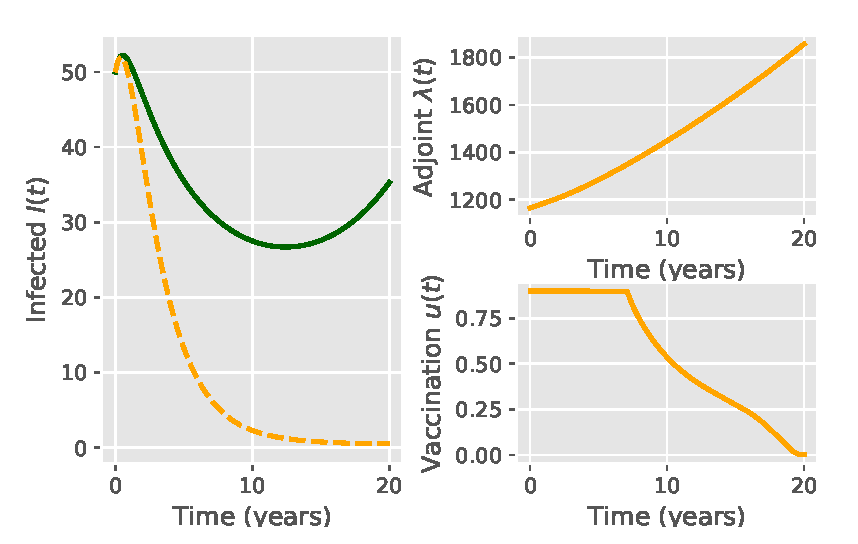
\includegraphics{./Figures/epidemics_lenhart_lab7}
	\caption{Likening between the controlled and uncontrolled Infected 
	 population.  At right, we show the optimal infected state agains the 
	 dynamics without 
	 control. At right we present the corresponding adjoint function $\lambda$ 
	 and the optimal control.}
\label{fig:epidemicslenhartlab7}
\end{figure}
